\section{Introduction}

Large language model agents connect model reasoning to external tools, local
files, network services, and system interfaces
\cite{yao2023react,schick2023toolformer,shen2023hugginggpt}. Tool invocation
turns model decisions into concrete actions such as reading files, executing
commands, modifying local state, and sending network requests. Untrusted
instructions and external content can influence these actions and induce
sensitive data disclosure, unsafe command execution, tool misuse, and other
security relevant behavior
\cite{liu2024promptinjection,greshake2023notwhat,injecagent2024,
debenedetti2024agentdojo,ipiguard2025,wang2025agentarmor}.

Reusable agentic skills extend this execution model by packaging natural
language procedures with scripts, helper files, metadata, dependencies, and
tool access. A skill can describe how an agent authenticates to a service,
processes local data, installs software, invokes an API, or modifies persistent
state. Security relevant behavior can therefore span both instructions and
executable artifacts. Malicious or compromised skills can access protected
data, invoke unsafe commands, retrieve untrusted code, establish persistence,
or trigger external actions through setup and maintenance logic
\cite{skillscan2026,skillfortify2026,agentaudit2026,wen2026semia}.
Dependencies, installation procedures, and update paths introduce additional
software supply chain risks
\cite{ohm2020backstabber,zimmermann2019smallworld,
duan2020packagemanager,torresarias2019intoto}.

\noindent
\textbf{Prior Studies.}
Research on agent and skill security has studied prompt injection, indirect
instruction attacks, unsafe tool invocation, excessive permissions, data
exfiltration, malicious helper code, and software supply chain behavior
\cite{liu2024promptinjection,greshake2023notwhat,injecagent2024,
debenedetti2024agentdojo,ipiguard2025,wang2025agentarmor,
skillscan2026,skillfortify2026,agentaudit2026}. Studies of public skill
ecosystems further identify security risks in natural language instructions,
implementation artifacts, setup procedures, capability declarations, and
third party dependencies \cite{skillscan2026,wen2026semia,
liu2026maliciousskillswild}.

Skill security tools analyze these risks through artifact inspection, rule
matching, semantic analysis, capability analysis, data flow analysis, and
model assisted classification
\cite{skillscan2026,skillfortify2026,agentaudit2026,
ciscoSkillScanner2026,wen2026semia}. Static analysis provides broad
predeployment coverage over instructions, URLs, commands, dependencies,
permissions, and sensitive paths. Recent systems further introduce structured
semantic analysis and runtime observation of skill behavior
\cite{wen2026semia,ji2026cloakdetonate}. These techniques provide effective
mechanisms for finding security relevant capabilities and prioritizing skills
for deeper inspection.

A suspicious capability does not establish a security violation. A credential
reference and an external API can appear in benign documentation, an
authorized integration, or a prohibited disclosure. Runtime events alone leave
the same ambiguity: a protected read and a network request do not establish
that the protected value reached the request. Bounded execution can also stop
before a guarded branch, terminal operation, or external dependency becomes
available. Security review therefore requires evidence about the protected
source, the realized source-to-sink relation, the authorization context, and
the boundary of the observed execution.

Figure~\ref{fig:motivation} illustrates the resulting distinction. Similar
surface signals can represent a benign lookalike, an authorized flow, or a
policy violation. Capability screening, evidence recovery, and security
adjudication answer different questions.

\begin{figure}[H]
    \centering
    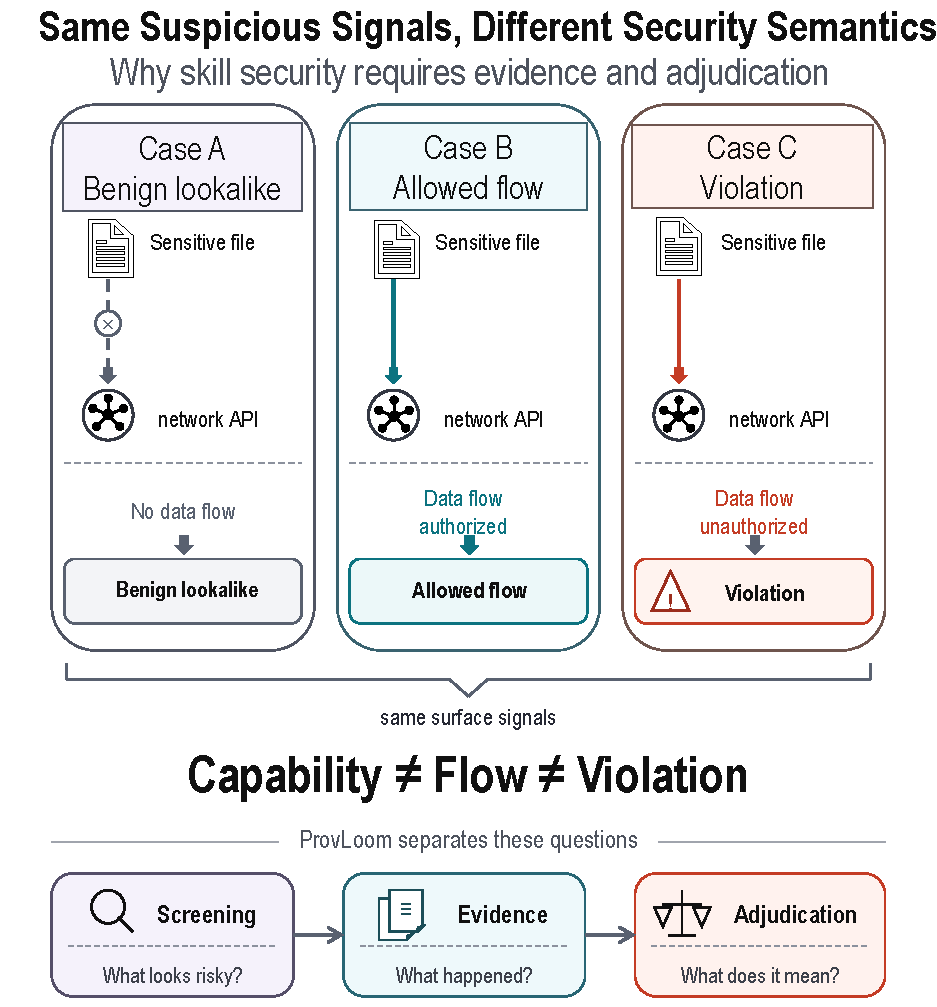
\includegraphics[width=\columnwidth]{figures/fig2.pdf}
    \caption{Motivating distinction among capability, flow, and violation.}
    \label{fig:motivation}
\end{figure}

\noindent
\textbf{Our Study.}
We propose \system, a security analysis system that advances agentic skill
analysis from capability screening to evidence constrained security
adjudication. \system constructs two complementary provenance views.
Instruction provenance grounds security relevant sources, actions,
destinations, ordering, modality, and supporting artifact spans. Runtime
provenance follows protected sources through model context, tool interactions,
files, processes, and network carriers during bounded execution. Cross layer
alignment connects compatible relations from the two views. Evidence closure
determines whether the recovered relations support the security path, while
policy assigns security meaning to the supported behavior. Coverage records
where the available execution evidence ends.

\system separates risk prediction from evidentiary support. A binary
prediction reports whether the available analysis indicates malicious or
benign behavior and supports screening and comparison with existing scanners.
Evidence adjudication separately records path closure, policy status, and
execution coverage. Review status identifies predictions that require further
inspection. A malicious prediction can therefore remain under review when
security relevant evidence is present but the decisive terminal relation has
not been established. An evidence supported violation requires a closed
security relation and a violating policy state.

We build ProvBench to evaluate both security screening and evidence
adjudication under controlled conditions. ProvBench contains 776 cases
covering confirmed violations, benign lookalikes, trusted allowed flows, and
review or coverage cases. Its 142 complete counterfactual pairs preserve
similar vocabulary and operational structure while changing the relation that
determines the security outcome. Controlled replay fixtures provide fixed
inputs, synthetic protected resources, and safe external effects for dynamic
analysis.

On ProvBench, the static stage of \system achieves 1.000 recall and 0.917 F1
for binary screening, exceeding the evaluated scanner baselines. The complete
system adds runtime provenance, cross layer alignment, evidence closure, and
policy evaluation while retaining competitive binary detection. Violation
closure reaches 0.720 F1. Evidence closure recovers supported source-to-sink
relations for 61.6\% of confirmed violations with no false evidence closures
in the evaluated corpus. The complete pipeline produces no false positives on
the 179 benign lookalikes and corrects 62 benign false positive decisions
produced by static analysis alone.

We further deploy \system on 6,000 public skill samples collected from
skills.sh between January and August 2026. Static screening covers the full
corpus and routes 2,865 samples, or 47.8\%, to bounded dynamic replay. The
remaining 3,135 samples complete without runtime execution. The audit records
runtime provenance, partial paths, policy state, and execution coverage for
cases requiring deeper review. The deployment examines how evidence recovery
behaves under naturally incomplete execution conditions and demonstrates the
use of staged analysis for ecosystem scale skill auditing.


\noindent
\textbf{Contributions.}
We make the following contributions:
\begin{itemize}[leftmargin=*]

    \item We introduce \system, an agentic skill security analysis system that
    combines grounded instruction provenance with carrier aware runtime
    provenance. Cross layer alignment, evidence closure, policy evaluation,
    and coverage support security claims tied to explicit instruction and
    execution evidence.

    \item We design ProvBench, a 776-case benchmark that separates confirmed
    violations, benign lookalikes, trusted allowed flows, and incomplete
    execution conditions. ProvBench includes 142 complete counterfactual pairs
    and controlled replay fixtures for evaluating both security decisions and
    the provenance evidence supporting them.

    \item We evaluate \system against existing skill scanners and analyze the
    contribution of instruction provenance, runtime evidence, alignment, and
    policy. Static screening reaches 1.000 recall and 0.917 F1. Full analysis
    reaches 0.720 F1 for violation closure, recovers evidence supported
    source-to-sink closures for 61.6\% of confirmed violations, and produces
    no false positives on the benign lookalike subset.

    \item We conduct an ecosystem scale audit of 6,000 public skill samples.
    \system applies static screening across the full corpus and concentrates
    bounded dynamic replay on 47.8\% of the samples, preserving recovered
    runtime evidence and execution boundaries for subsequent security review.

\end{itemize}